\documentclass[a4paper]{article}    % define document layout
%\documentclass[draft]{article}     % use draft option in packages
%-----------------------------
% preamble
%-----------------------------
\usepackage[sumlimits,]{amsmath}    % math equations and formulas
\usepackage[utf8]{inputenc}         % use UTF-8 encoding
\usepackage[english]{babel}         % use English language
\usepackage{graphicx}              % insert images
%\usepackage[draft]{graphicx}        % do not render figures
\usepackage{subcaption}             % multiple images in one figure
\usepackage{hyperref}               % hyperlinks
\usepackage{float}                  % floating objects (figures, tables)
\usepackage{geometry}               % page size and margins
\geometry{a4paper, margin=1in}      % margins
\usepackage{ragged2e}               % text alignment
%\usepackage{multirow}               % merge rows in table

\graphicspath{                      % path for figures
    {../figures/} 
    {../figures/pre-ex1/} 
    {../figures/ex1/} 
    {../figures/ex2-multiclass_classification/} 
    {../figures/ex2-knn/} 
}

%-----------------------------
% body
%-----------------------------
\begin{document}

\begin{figure}
    \centering
    % UNICAMP logo
    \begin{subfigure}{0.45\textwidth}
        \centering
        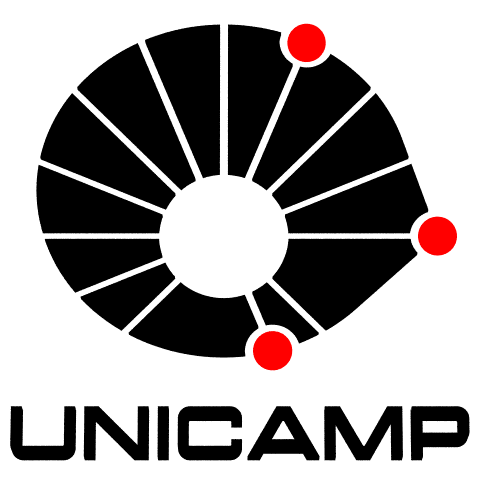
\includegraphics[width=1.5cm]{unicamp}
%        \label{fig:unicamp}
    \end{subfigure}
    \hfill
    % FEEC logo
    \begin{subfigure}{0.45\textwidth}
        \centering
        
\includegraphics[width=1.5cm]{feec}
%        \label{fig:feec}
    \end{subfigure}
\end{figure}

\title{EFC3 - Exercise 3}
\author{Rafael Claro Ito (R.A.: 118430)}
%R.A.: 118430
%ito.rafael@gmail.com
\date{November 2019}
\maketitle
\newpage

%=================================================
\section{Source files}
%=================================================

\paragraph{All code cited and all figures showed here can be found at the following GitHub repository:\\
\url{https://github.com/ito-rafael/IA006C-MachineLearning/tree/master/efc2}\\
In this repository, one can found the following files:\\}

\begin{itemize}
    \item Jupyter Notebook
    \begin{itemize}
        \item \href{https://github.com/ito-rafael/IA006C-MachineLearning/blob/master/efc2/efc2_pre-ex1.ipynb}{efc2\_pre-ex1.ipynb}
        \item \href{https://github.com/ito-rafael/IA006C-MachineLearning/blob/master/efc2/efc2_ex1_binary_classification.ipynb}{efc2\_ex1\_binary\_classification.ipynb}
        \item \href{https://github.com/ito-rafael/IA006C-MachineLearning/blob/master/efc2/efc2_ex2_multiclass_classification.ipynb}{efc2\_ex2\_multiclass\_classification.ipynb}
        \item \href{https://github.com/ito-rafael/IA006C-MachineLearning/blob/master/efc2/efc2_ex2_knn.ipynb}{efc2\_ex2\_knn.ipynb}
    \end{itemize}
    \item \LaTeX
    \begin{itemize}
        \item \href{https://github.com/ito-rafael/IA006C-MachineLearning/blob/master/efc2/LaTeX/efc2.tex}{efc2.tex}
    \end{itemize}
\end{itemize}

\paragraph{The notebook ``efc2\_pre-ex1'' plots the histograms for the exercise 1 and it is used for data visualization. It shows the input features histograms for the raw data and after a data standardization. Also, it shows the correlation between these data.}

\paragraph{The notebook ``efc2\_ex1\_binary\_classification'' effectively implements the logistic regression used to perform a binary classification proposed in exercise 1.}

\paragraph{The notebooks ``efc2\_ex2\_multiclass\_classification'' and ``efc2\_ex2\_knn'' implements the algorithms to perform a multiclass classification proposed in exercise 2. The former one uses the softmax approach while the latter one implements the K-Nearest Neighbors (kNN) algorithm.}

\bigskip

%=================================================
\section{Part 1 - Error backpropagation}
%=================================================

$ u_1 = 1 \cdot v_{00} + x_1 \cdot v_{10} + x_2 \cdot v_{20} $\\
$ u_2 = 1 \cdot v_{01} + x_1 \cdot v_{11} + x_2 \cdot v_{21} $\\
$ u_3 = 1 \cdot v_{02} + x_1 \cdot v_{12} + x_2 \cdot v_{22} $\\
\vspace{0.1mm}\\
$ s_1 = f(u_1) $\\
$ s_2 = f(u_2) $\\
$ s_3 = f(u_3) $\\
\vspace{0.1mm}\\
$ y_1 = 1 \cdot w_{00} + s_1 \cdot w_{10} + s_2 \cdot w_{20} + s_3 \cdot w_{30} $\\
$ y_2 = 1 \cdot w_{01} + s_1 \cdot w_{11} + s_2 \cdot w_{21} + s_3 \cdot w_{31} $\\
\vspace{0.1mm}\\
$ J = e_1^2 + e_2^2 $\\
\vspace{0.1mm}\\
$ \delta_3 = \dfrac{\partial J}{\partial u_3} = \dfrac{\partial [(d_1-y_1)^2+(d_2-y_2)^2]}{\partial u_3} $\\
$ \delta_3 = \dfrac{\partial (d_1-y_1)^2}{\partial u_3} + \dfrac{\partial (d_2-y_2)^2}{\partial u_3} $\\
$ \delta_3 = \dfrac{\partial (d_1-y_1)^2}{\partial (d_1-y_1)} \cdot \dfrac{\partial (d_1-y_1)}{\partial u_3} + \dfrac{\partial (d_2-y_2)^2}{\partial (d_2-y_2)} \cdot \dfrac{\partial (d_2-y_2)}{\partial u_3} $\\
$ \delta_3 = 2(d_1-y_1) \cdot \left(-\dfrac{\partial y_1}{\partial u_3}\right) + 2(d_2-y_2) \cdot \left(-\dfrac{\partial y_2}{\partial u_3}\right) $\\
$ \delta_3 = - 2(d_1-y_1) \cdot \dfrac{\partial y_1}{\partial s_3} \cdot \dfrac{\partial s_3}{\partial u_3} - 2(d_2-y_2) \cdot \dfrac{\partial y_2}{\partial s_3} \cdot \dfrac{\partial s_3}{\partial u_3} $\\
$ \delta_3 = - 2(d_1-y_1) \cdot \dfrac{\partial (1 \cdot w_{00} + s_1 \cdot w_{10} + s_2 \cdot w_{20} + s_3 \cdot w_{30})}{\partial s_3} \cdot \dfrac{\partial f(u_3)}{\partial u_3} - 2(d_2-y_2) \cdot \dfrac{\partial (1 \cdot w_{01} + s_1 \cdot w_{11} + s_2 \cdot w_{21} + s_3 \cdot w_{31})}{\partial s_3} \cdot \dfrac{\partial f(u_3)}{\partial u_3} $\\
$ \delta_3 = - 2(d_1-y_1)\dot{f}(u_3)w_{30} - 2(d_2-y_2)\dot{f}(u_3)w_{31} $\\
\vspace{0.1mm}\\
$ \dfrac{\partial J}{\partial v_{12}} = \dfrac{\partial J}{\partial u_3} \cdot \dfrac{\partial u_3}{\partial v_{12}} $\\
$ \dfrac{\partial J}{\partial v_{12}} = \dfrac{\delta_3 \cdot \partial(1 \cdot v_{02} + x_1 \cdot v_{12} + x_2 \cdot v_{22})}{\partial v_{12}} $\\
$ \dfrac{\partial J}{\partial v_{12}} = \delta_3 \cdot x_1 $\\
$ \dfrac{\partial J}{\partial v_{12}} = -2x_1\dot{f}(u_3)[w_{30}(d_1-y_1) + w_{31}(d_2-y_2)] $\\
\vspace{0.1mm}\\

%=================================================
\section{Part 2 - Multiclass Classification}
%=================================================

%=================================================
\end{document}
